\chapter{Introduction}
\label{ch:introduction}

\section{Motivation}

Hybrid VTOLs are particularly interesting vehicle to study, which has an intermediate mode as either a Multirotor, or a Fixed Wing. However, conventional path following algorithms fail to incorporate both modes of operation.

\subsection*{Limitations of Conventional Path Following Guidance}

Currently, conventional path following algorithms suffer from the following two problems:

\begin{figure}[h]
  \begin{minipage}[t]{0.48\textwidth}
    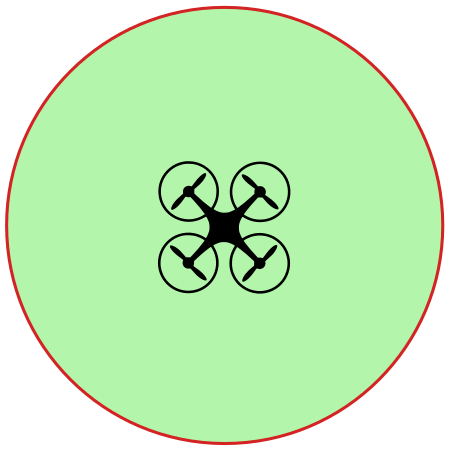
\includegraphics[width = \textwidth]{MC_Velocity_Range_v2}
  \end{minipage}
  \hfill
  \begin{minipage}[t]{0.48\textwidth}
    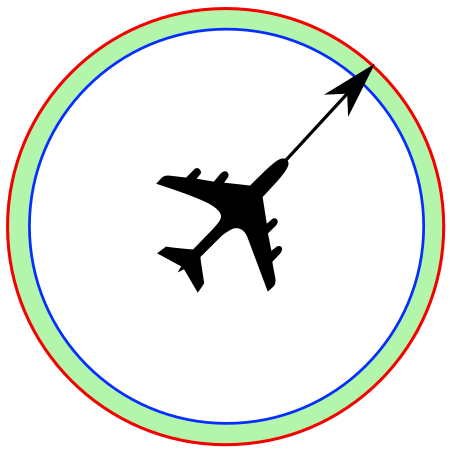
\includegraphics[width = \textwidth]{FW_Velocity_Range_v2}
  \end{minipage}
  \caption{Permittable Velocity Range (in green) for the Multirotor and Fixed wing vehicles (Maximum shown in Red, Minimum in Blue)}
  \label{pics:cycle}
\end{figure}

\begin{enumerate}
    \item \textbf{Constant nominal speed}: Both multirotor and fixed wings are expected to execute path following at a constant speed
    \item \textbf{Definition of the nominal speed}: For a fixed wing vehicles, it makes sense to define the nominal speed as it's energy optimal cruise flight speed, but for multirotors there is no equivalent concept
\end{enumerate}

In fact, when we try out the conventional fixed wing path following algorithm on an agile platform like multirotor, it exhibits a sub-optimal characteristics such as:

\begin{enumerate}
    \item \textbf{Limited agility}: Since fixed wing vehicles are very slow, the path following guidance didn't account for the agility multirotors can have. Thus, the guidance output is much less aggressive than we desire.
    \item \textbf{Limited velocity profile}: As the guidance algorithm assumes a constant speed while following a path, we lose the ability to freely manipulate the magnitude of the velocity.
\end{enumerate}

\section{Definitions}
Here the definitions for the terminologies are formulated alongside the graphic.

\begin{figure}[h]
\centering
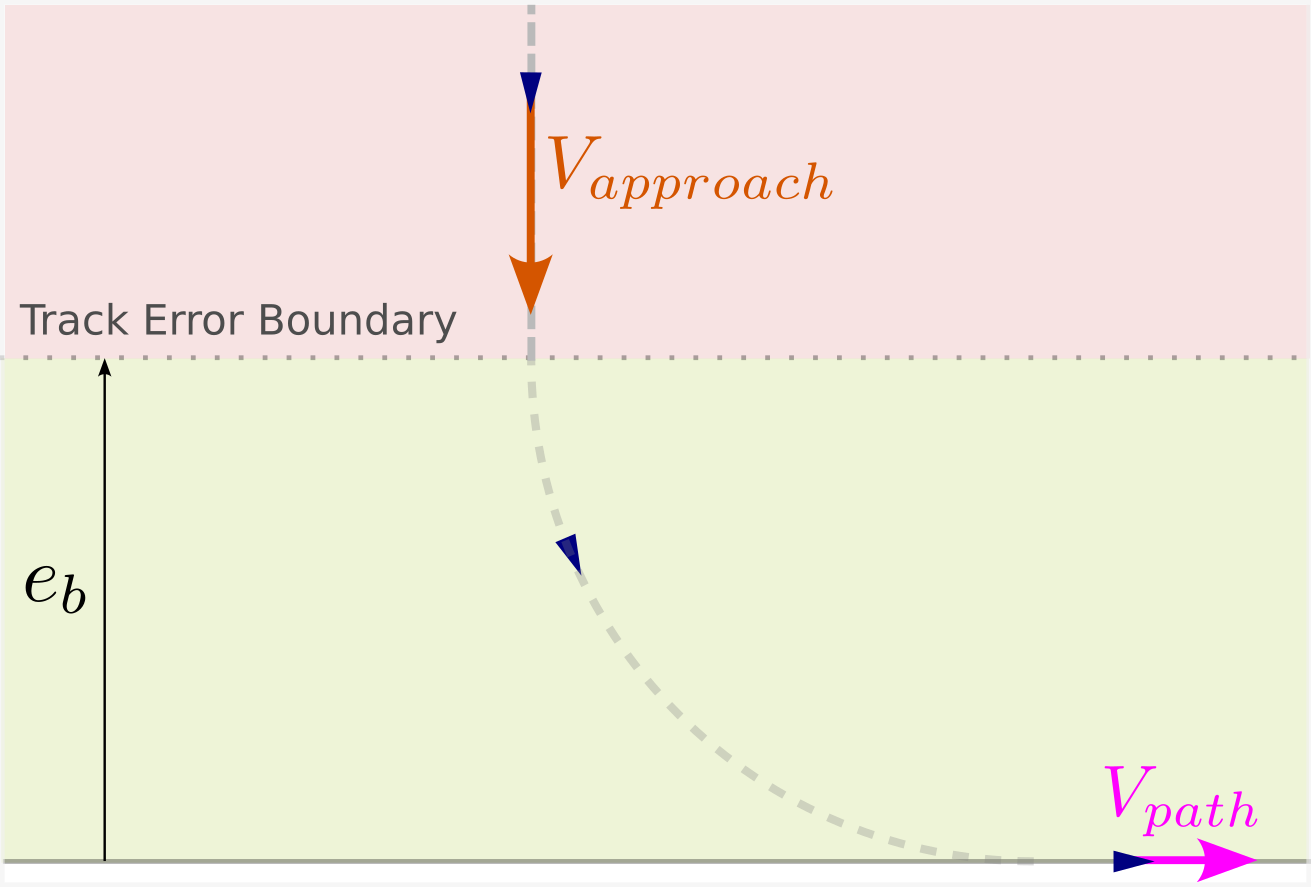
\includegraphics[width=\textwidth]{PathFollowing_Problem_v2_arrow_enlarged_simplified}
\caption{Path Following Terminology Definition}
\end{figure}

The path following is divided into three phases

\begin{enumerate}
    \item \textbf{Approach}: When sufficiently far away from the path, vehicle approaches to the closest point on path in a direction orthogonal to path at an approach speed $V_{approach}$
    \item \textbf{Turning}: After vehicle crosses the track error boundary $e_b$, it starts to turn onto the path, diminishing the orthogonal velocity component
    \item \textbf{On-path}: When on path (moderately close), vehicle follows the path at a specified on-path speed $V_{path}$ in the direction of unit tangent vector $\hat{t_p}$
\end{enumerate}

In practice, most path-following algorithms focus on the second phase, 'Turning'. Since when on or far from path, vehicle has a relatively simple velocity setpoint to follow (follow or approach). Numerous solutions were suggested for the Turning phase in the past, which is summarized in \autoref{ch:related_work}.\\

And the formulations for path-following algorithms is essentially coming up with how to control (velocity, acceleration, position, angular rate, etc) the vehicle to achieve a satisfactory Turning phase.\\

Furthermore, the terms are defined more rigorously.

\begin{equation}
    \overline{e} = constrain(\frac{||e||}{e_b}, 0, 1)
\label{eq:normliazed_track_error_def}
\end{equation}

\section{Assumptions}
Throughout the

\section{Goal of this Project}
The goal of this thesis is to construct a unified path following guidance that can be utilized both by Multirotor and Fixed Wing vehicles, thereby also allowing the usage on Hybrid VTOL vehicles.

\section{Contributions}
This thesis, to our best knowledge, describes the first unified path following guidance that specifically accounts for the maneuverability envelope of a Hybrid VTOL.

\section{Overview}
This thesis is structured as following:

\begin{enumerate}
    \item In \ref{ch:problem_definition}{Problem Definition}, we examine the path following problem in detail, and come up with the terminologies as well as the constraints that needs to be respected
    \item In Methods, we present 3 different formulations including the base method (from a past publication) and discuss the differences between them
    \item In Evaluation, we evaluate the formulations against the constraints and desired characteristics defined before
    \item In Conclusion, we determine which formulation is the best, and the use cases based on the evaluation
\end{enumerate}